% ! TeX root = ./document.tex
\documentclass[8pt, aspectratio=169, handout]{beamer}
% ! TeX root = ../document.tex
\usepackage[utf8]{inputenc}
\usepackage{multicol}
\usepackage{pgfpages}
\usepackage{roboto}
\usepackage{PlayfairDisplay}
\usepackage{fontawesome5}
\usepackage[T1]{fontenc}
\usepackage[final]{pdfcomment}
\usepackage{minted}
\usepackage[backend=bibtex,style=alphabetic,sorting=none,doi=true,url=false]{biblatex} 
\usepackage{xargs}
% ! TeX root = ../document.tex
\usetheme{material}
\useDarkTheme
\usePrimaryRed
\useAccentGreen

% ! TeX root = ../document.tex

\title{
  {\fontfamily{\playfairfamily}\fontseries{black}\selectfont
    Towards Reinforcement Learning-based \\ Aggregate Computing
  }
}
\author[G.Aguzzi]{
  \textbf{Gianluca Aguzzi}\inst{1}, Roberto Casadei \inst{1}, Mirko Viroli \inst{1}
}
\institute{
  \inst{1}
  \texttt{Alma Mater Studiorum} -- Università di Bologna, Cesena, Italy
}
\talk{
  Talk @ COORDINATION 2022
}

\bibliography{biblio.bib}
\begin{document}
\begin{frame}[plain]
  \begin{backgroundblock} 
    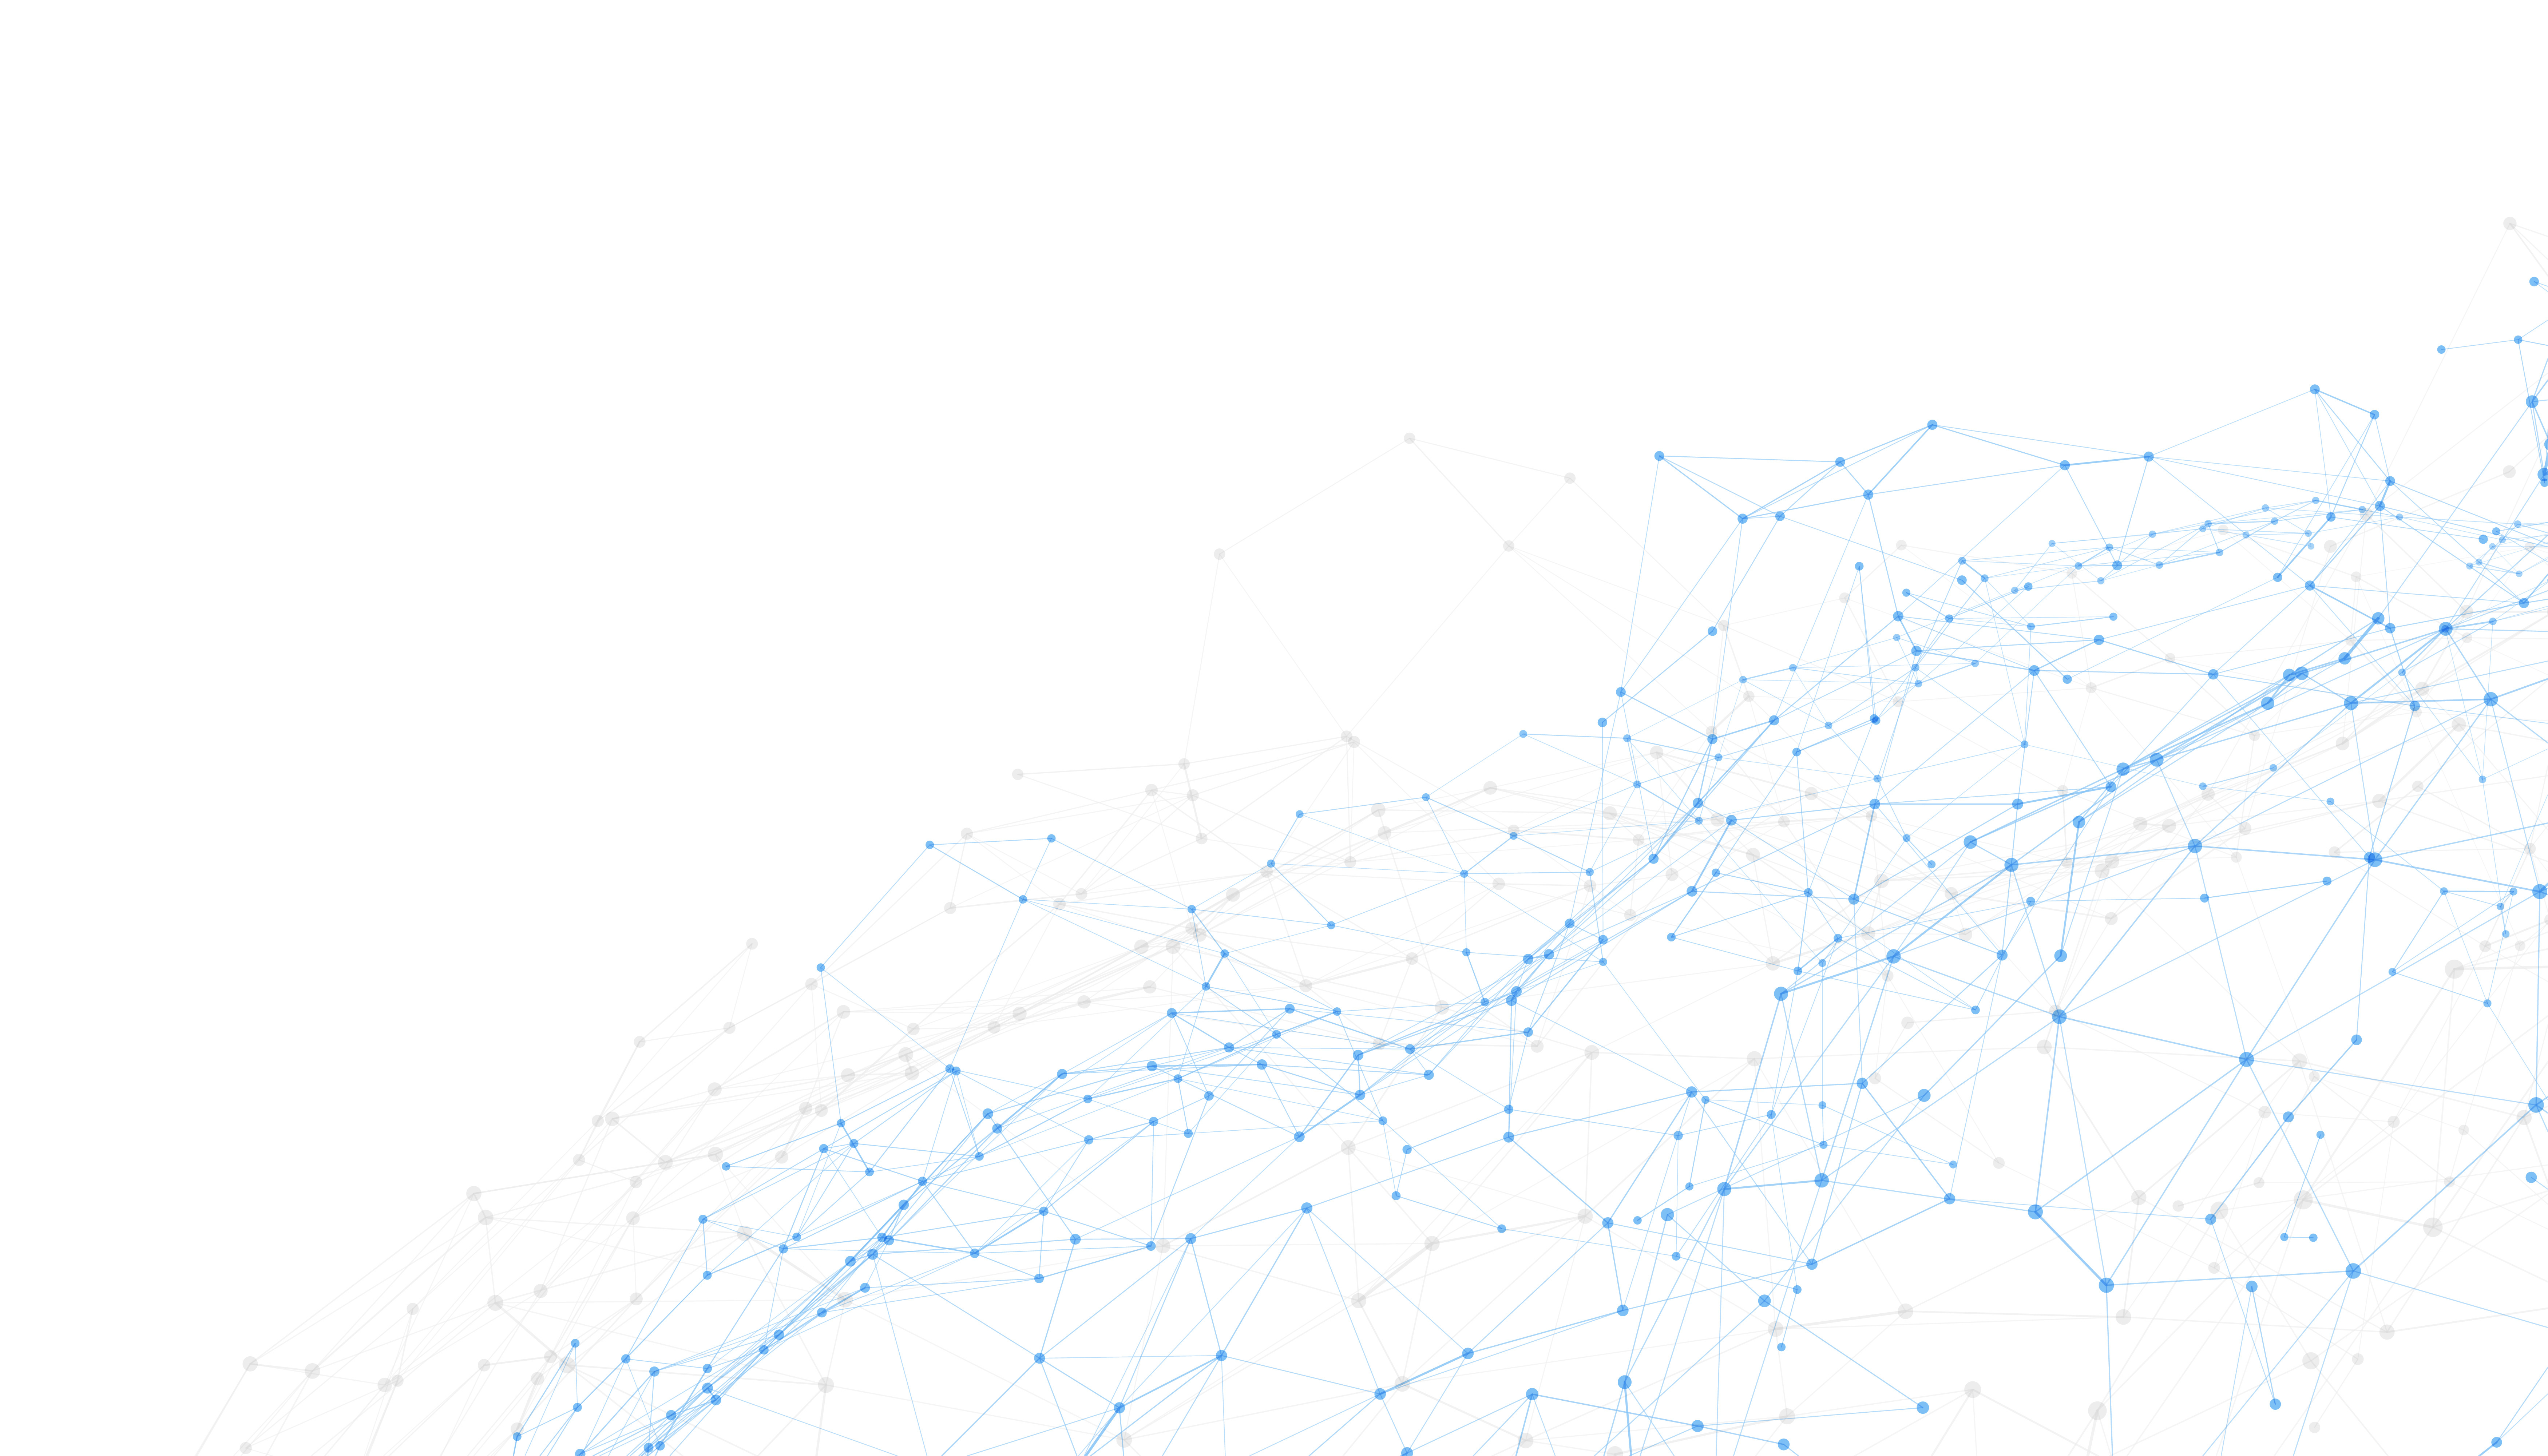
\includegraphics[width=\paperwidth]{img/network.jpg} 
  \end{backgroundblock} 
\titlepage
\end{frame}
\addtocounter{framenumber}{-1}
\section{Background}
\begin{frame}{Collective/Complex Adaptive Systems}
  \begin{card}[The systems of today!]
    \begin{itemize}
      \item [\faArrowRight] \emph{Context:} Dynamic Envirnoments + Large Scale Network of Cyber-Physical entities
      \item [\faArrowRight] \emph{Global Interpretation:} embedded devices collectively form a ``diffused'' computational systems
      \item [\faArrowRight] \emph{Examples}: Pervasive Systems, Drone swarms, Smart cities/building, \dots
    \end{itemize}
  \end{card}
  \centering
  \begin{multicols*}{3}
    \cardImg{img/queen}{0.30\textwidth}   
    \cardImg{img/traffic}{0.30\textwidth} 
    \cardImg{img/swarm}{0.30\textwidth} 
  \end{multicols*}
\end{frame}
\begin{frame}{Application Examples: Crowd Engineering}
  \begin{multicols*}{3}
    \begin{card}[Crowd-Detection]
      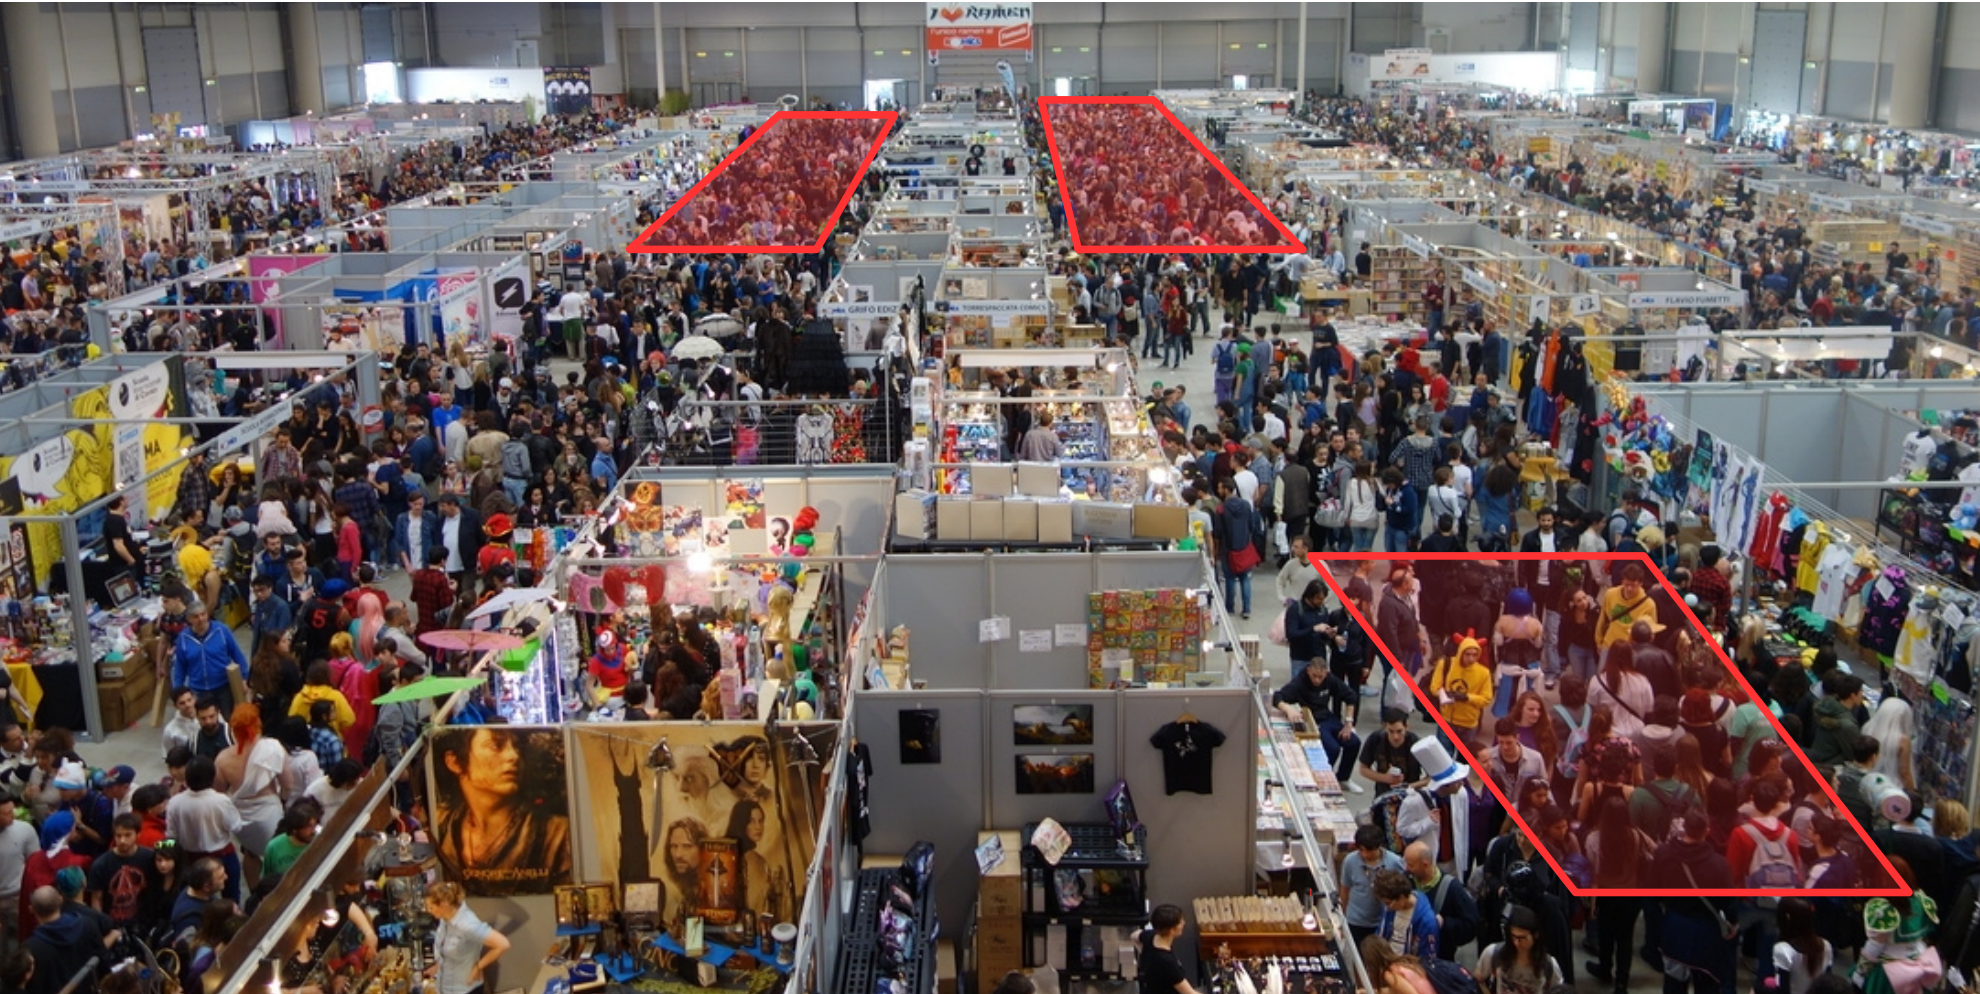
\includegraphics[width=\textwidth]{img/crowd-detection.png}
    \end{card}
    \begin{card}[Crowd-Aware steering]
      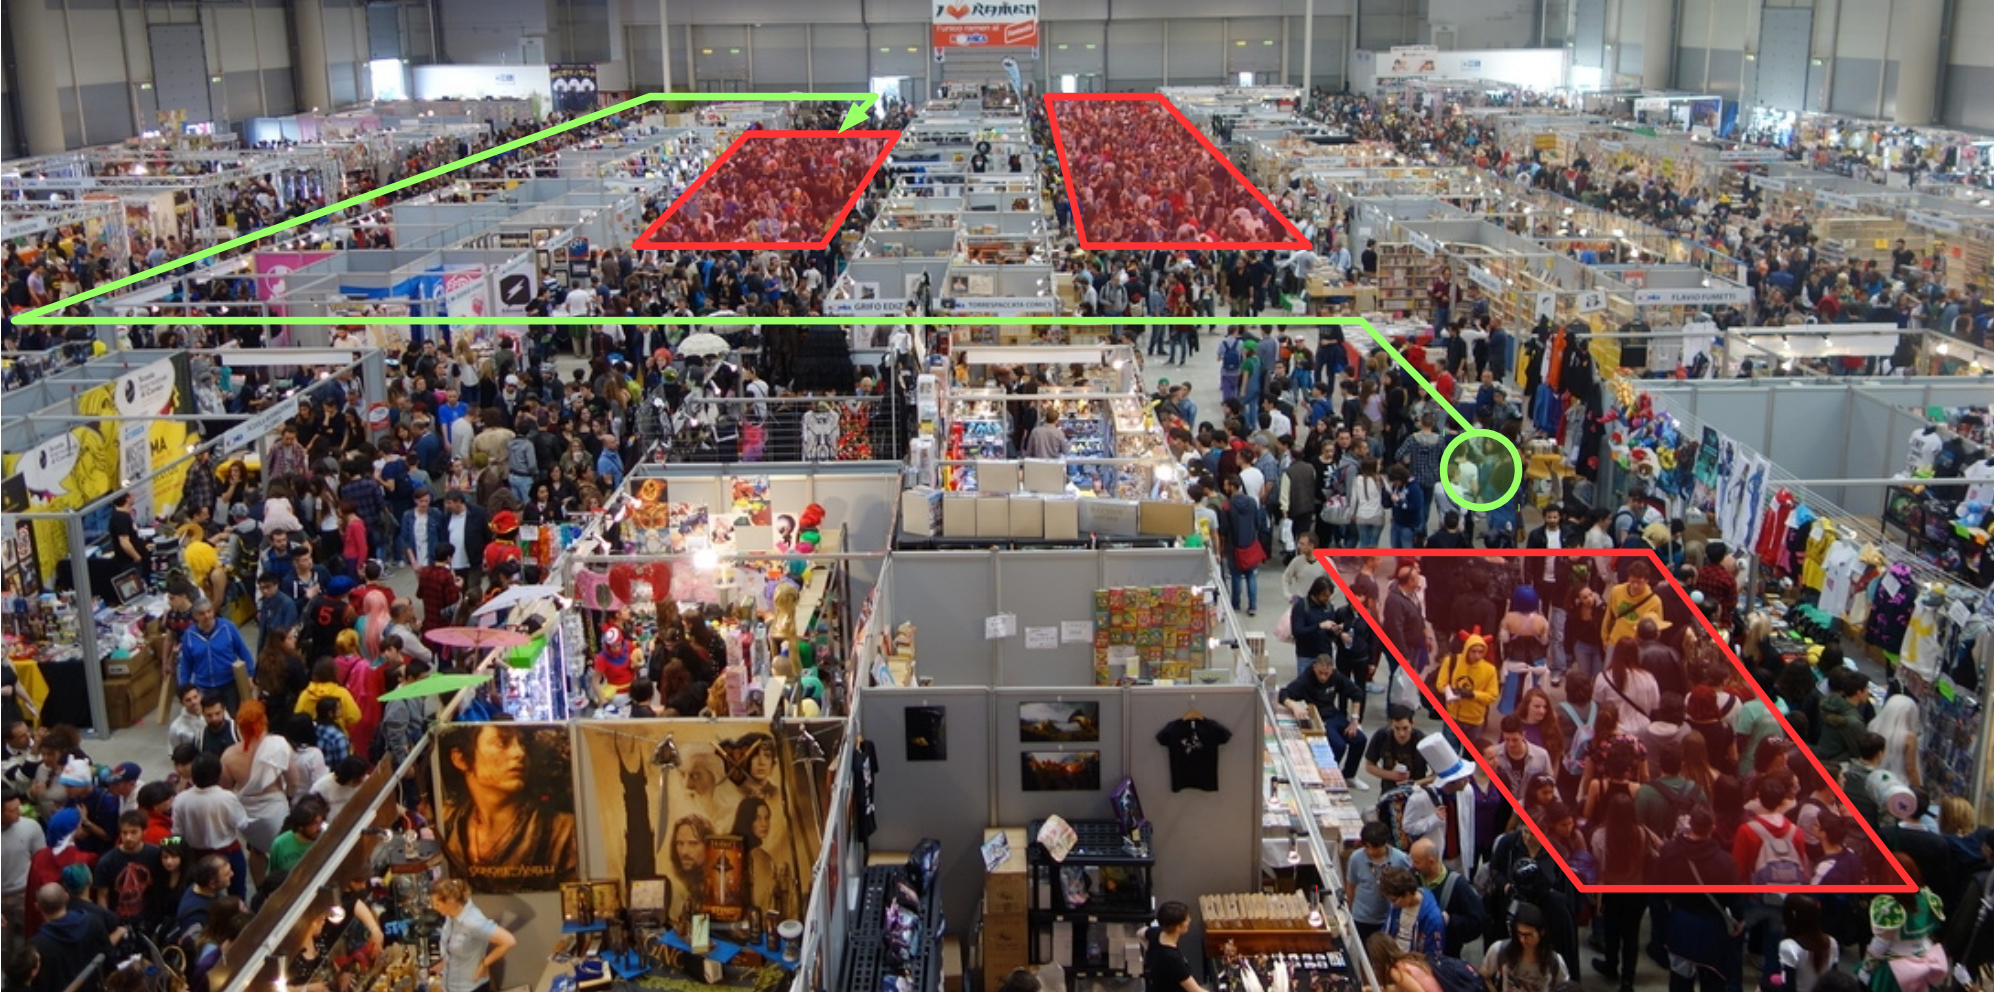
\includegraphics[width=\textwidth]{img/crowd-steering.png}
    \end{card}
    \begin{card}[Contact Tracing]
      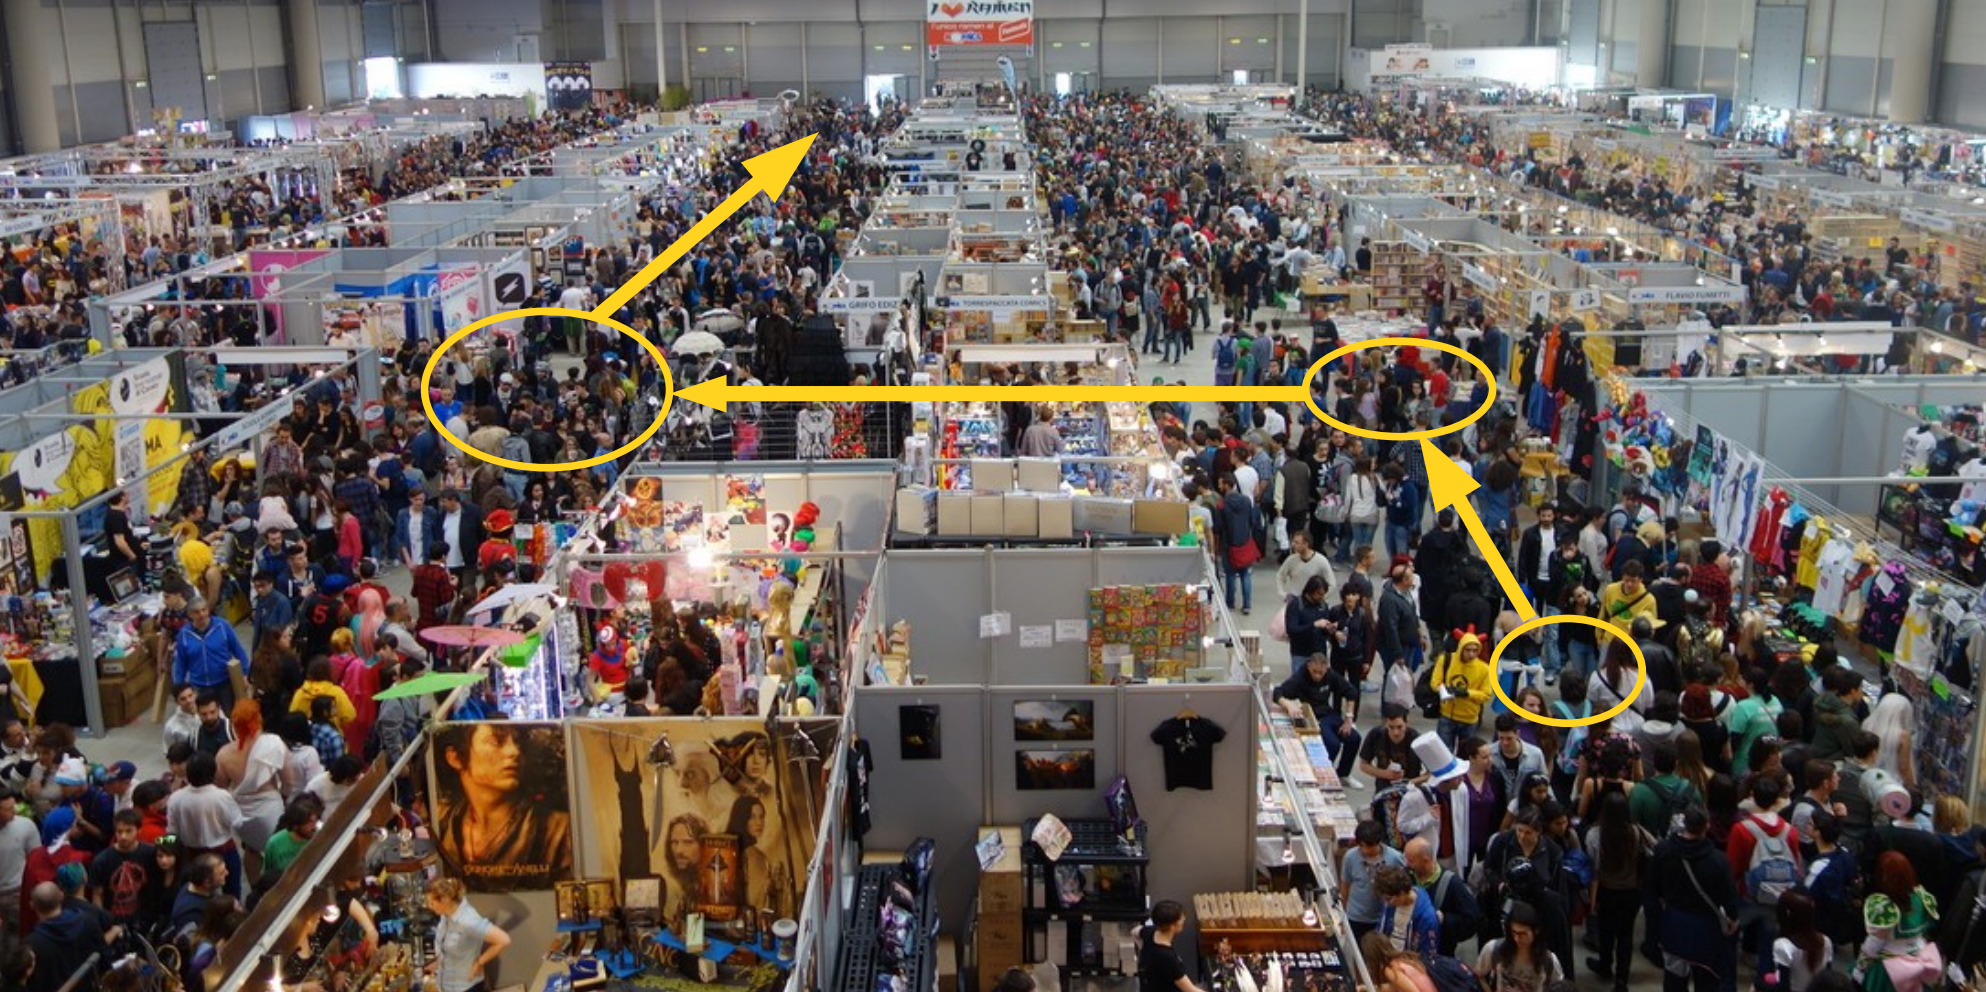
\includegraphics[width=\textwidth]{img/contact-tracing.png}
    \end{card}
    
  \end{multicols*}
\end{frame}
\begin{frame}{Design/Program CASs applications}
  \begin{alarm}[Challenges: worst case scenario]
    \begin{itemize}
      \item \emph{Zillion} of devices \emph{unpredictabily} located and moving in the environement
      \item Heterogenous displacement, \emph{pervasive} sensing/actuation
      \item Computational service are mostly \emph{contextual} (i.e., proximity based)
      \item \emph{Complex} \& \emph{layered} IT infrastructures (edge/fog/cloud computing)
      \item[\faArrowRight] What are the right abstractions/programming model for such a kind of systems?
    \end{itemize}
  \end{alarm}
  \begin{card}[A possible good abstractions/model]
    \begin{itemize}
      \item[\faThumbsUp] Abstract from individual devices program, low-level interaction protocol, and environement details
      \item[\faThumbsUp] Focus on how the \emph{global output} pattern can be obtained from global
      inputs
      \item[\faThumbsUp] Focus on both spatial and temporal computing patterns
      \item[\faThumbsUp] Refer to an abstract notion of executing platform, easily adaptable to
      real-life contexts (\emph{reality gap}) 
    \end{itemize}
  \end{card}
\end{frame}
\section{Aggregate Computing}

\begin{frame}{Aggregate Computing}
  \begin{card}[Motto: \emph{program the aggregate, not the individual devices}]
    \begin{itemize}
      \item \highlight{The reference computing machine}
      \faArrowRight \, an aggregate of devices as single ``body'', fading to the actual space
      \item \highlight{The reference elaboration process}
      \faArrowRight \,  atomic manipulation of a collective data structure (a so-called \emph{field})
      \item \highlight{The actual networked computation}
      \faArrowRight \, a proximity-based self-organisation system hidden “under-the-hood”
    \end{itemize}
  \end{card}
  \centering
  \cardImg{img/ac.png}{0.5\textwidth}
\end{frame}
\begin{frame}[allowframebreaks]{Computational Fields}
  \begin{card}[Traditionally a map: Space \faArrowRight \, Values]
    \begin{itemize}
      \item Possibly: evolving over time, dynamically injected, stabilising
      \item Smoothly adapting to very heterogeneous domains
      \item More easily ``understood'' on continuous and flat spatial domains
      \item Ranging to: booleans, reals, vectors, functions
    \end{itemize}
    
  \end{card}
  \centering
  \begin{multicols}{3}
    \begin{card}[Numeric partition in 2D]
      \centering
      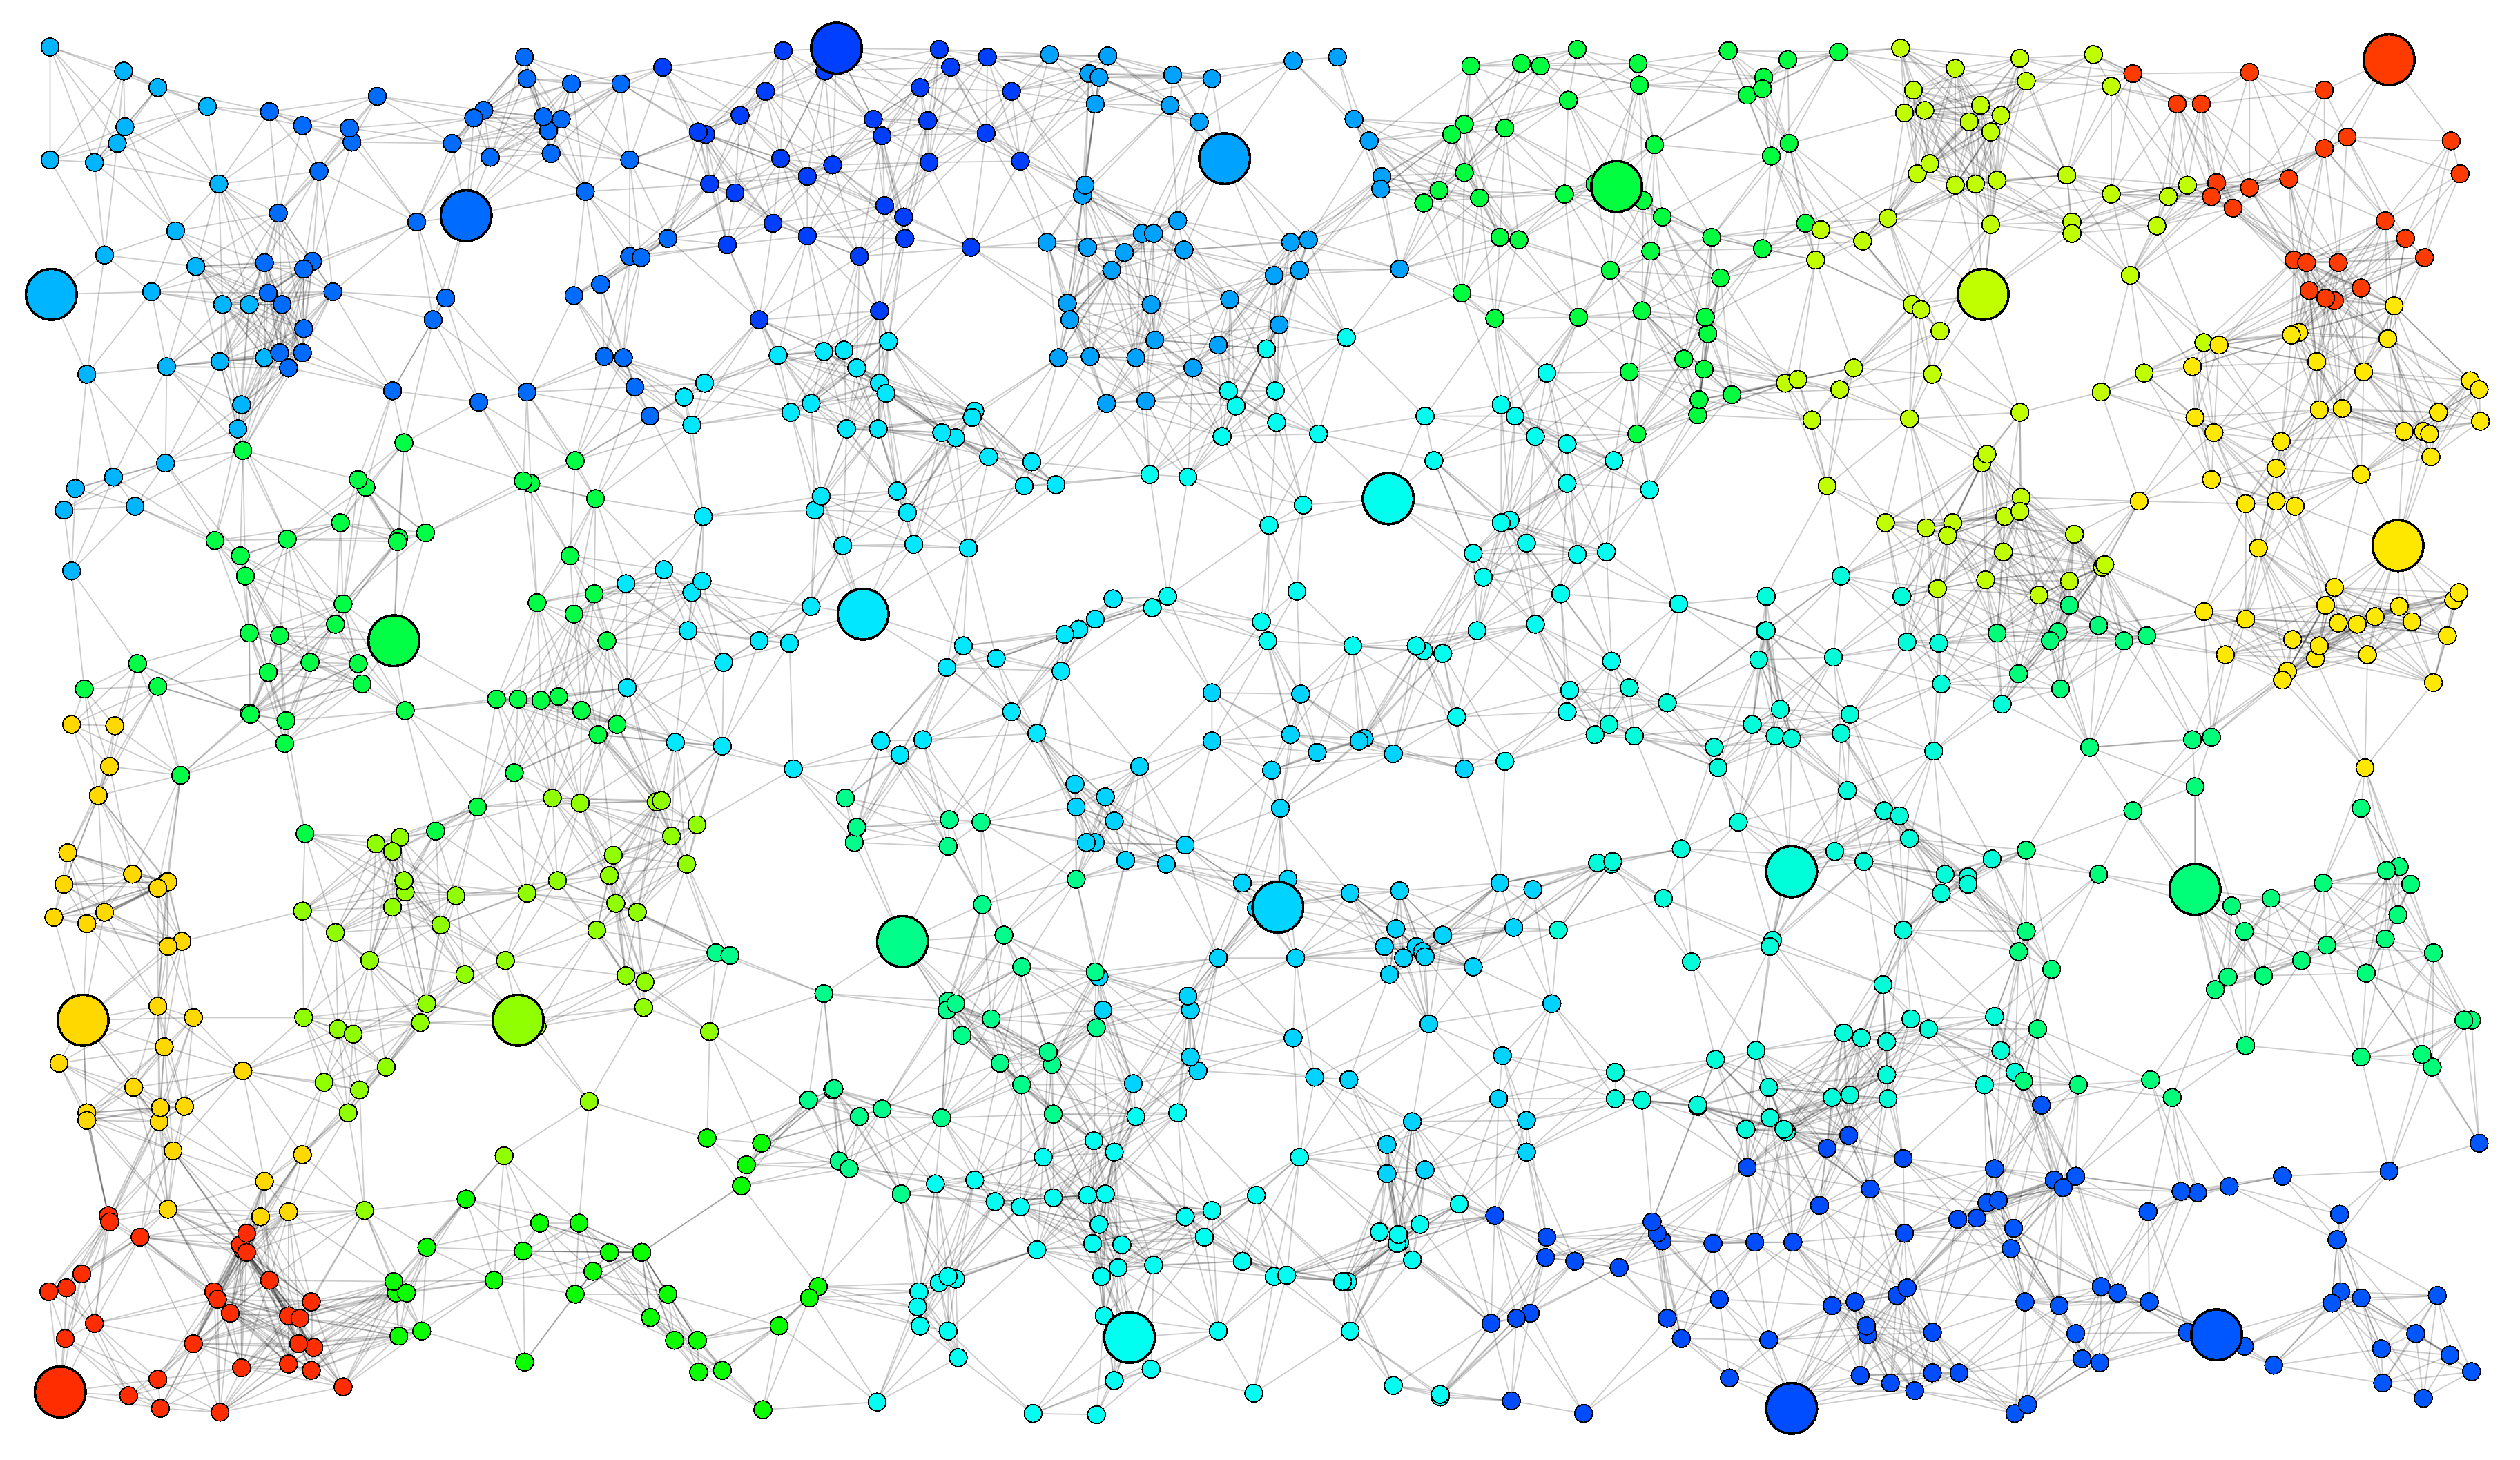
\includegraphics[height=15mm]{img/scr-result.png}
    \end{card}
    \begin{card}[Boolean field in 2D]
      \centering
      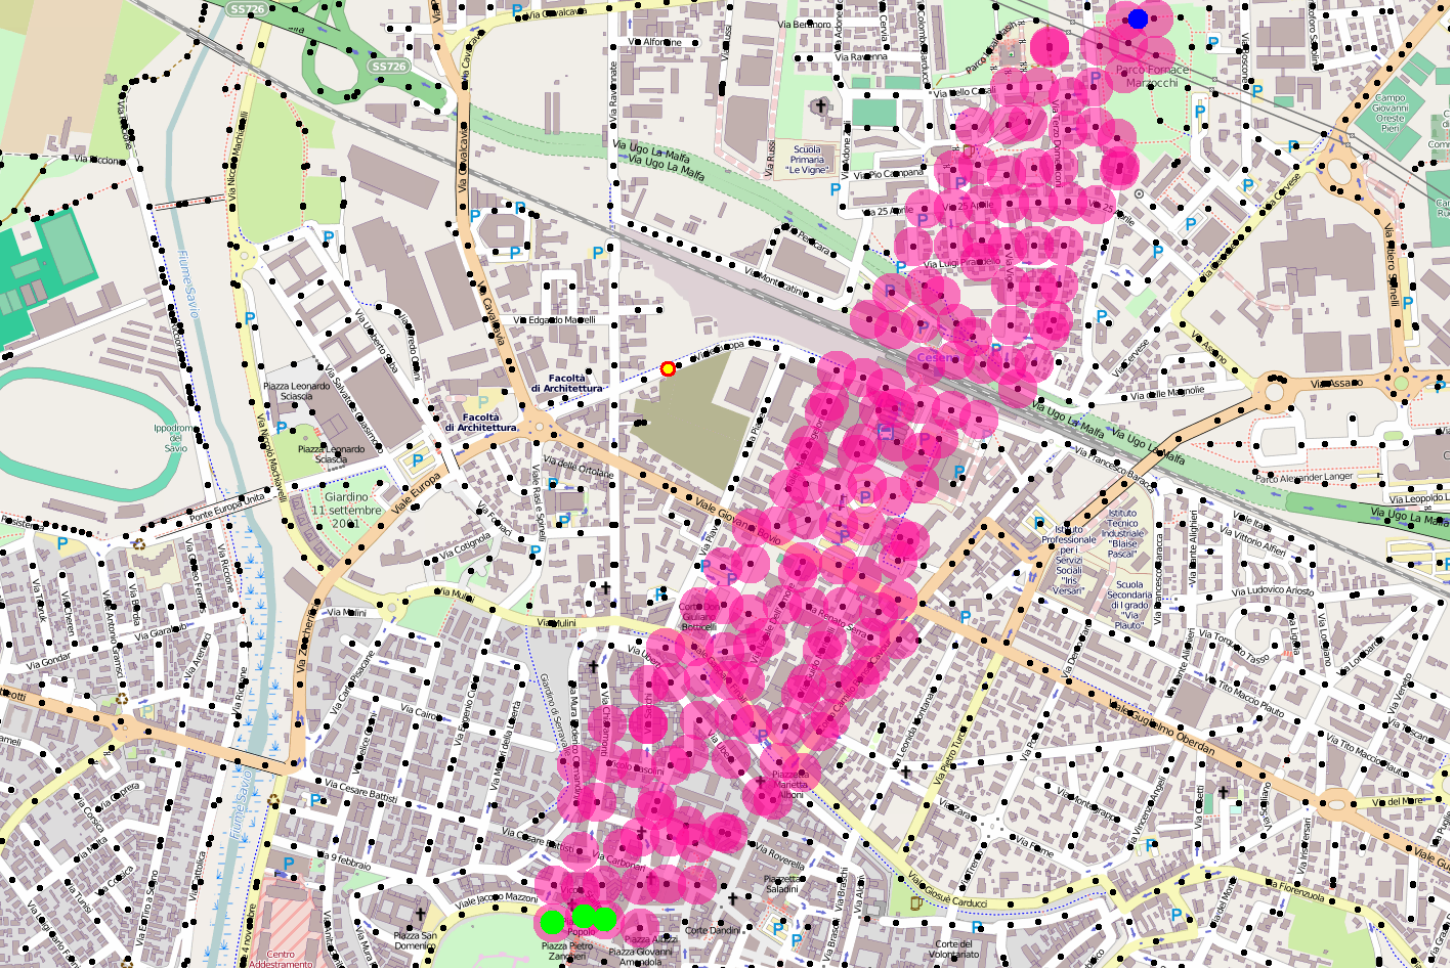
\includegraphics[height=15mm]{img/channel.png}
    \end{card}
    \begin{card}[Real-value gradient in 3D]
      \centering
      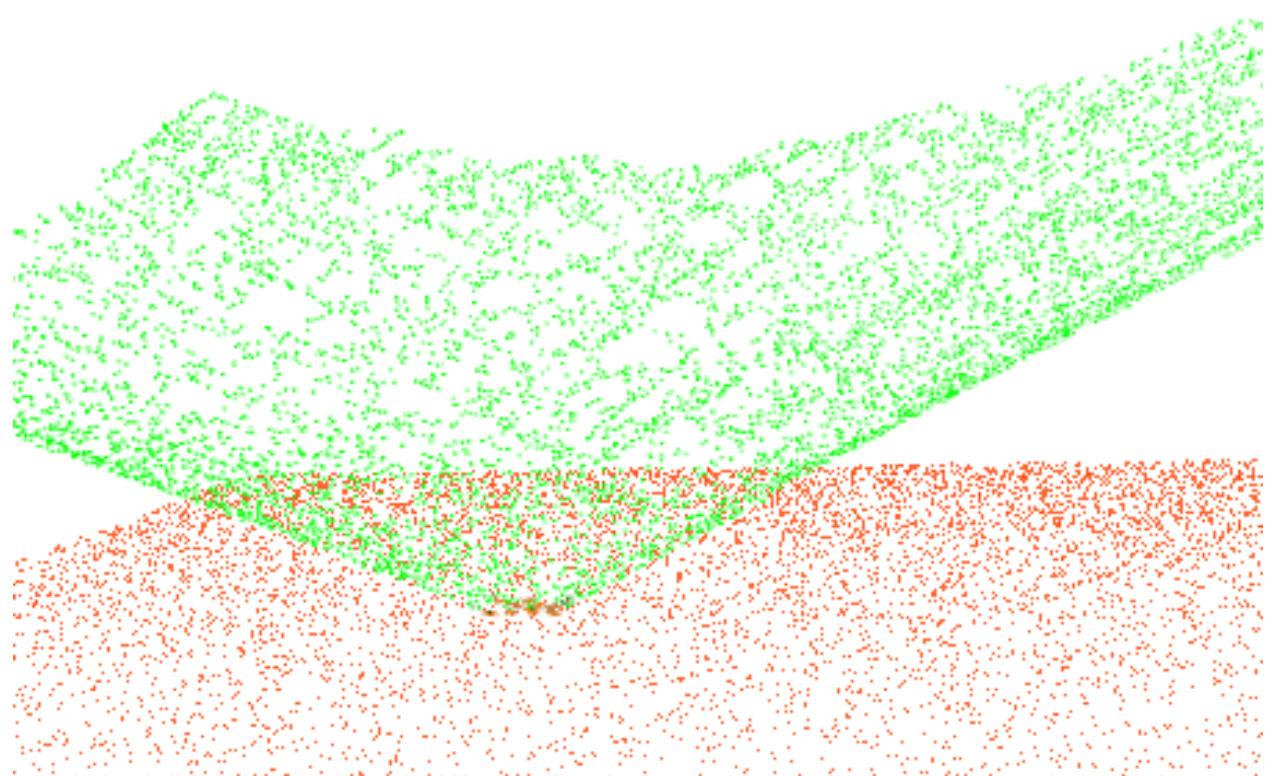
\includegraphics[height=15mm]{img/3d-gradient.png}
    \end{card}
  \end{multicols}
  \begin{card}[Nowadays: a space-time structure: $\phi \, : \, D \rightarrow V$]
    \begin{itemize}
      \item \emph{event $E$}: a triple $\langle\delta, t, p\rangle$ – device $\delta$, ``firing" at time $t$ in position $p$
      \item \emph{events domain $D$}: a coherent set of events (devices cannot move too fast)
      \item \emph{field values $V$}: any data value
    \end{itemize}
  \end{card}
  \centering
  \begin{multicols}{2}
    \cardImg{img/left-space-time-field.png}{0.3\textwidth}
    \cardImg{img/right-space-time-field.png}{0.3\textwidth}
  \end{multicols}
\end{frame}
\begin{frame}{An example problem: computing a route towards a POI}
  \centering
  \cardImg{img/channel.png}{0.7\textwidth}
\end{frame}

\begin{frame}{Aggregate programming as a functional approach}
  \begin{card}[Functionally composing fields]
    \begin{itemize}
      \item Inputs: sensor fields, Output: actuator field (e.g., alarm, velocity, ...)
      \item Computation is a pure function over fields (time embeds state!)
      \item[\faArrowRight] for this to be practical/expressive we need a good programming language
    \end{itemize}
  \end{card}
  \centering
  \cardImg{img/composition.png}{0.4\textwidth}
\end{frame}
\begin{frame}[fragile, allowframebreaks]{Computing with Fields}
  \begin{card}[Field/aggregate computation in scala: ScaFi]
    \begin{minted}{scala}
trait Constructs:
  def rep[A](init: => A)(fun: A => A): A
  def nbr[A](expr: => A): A
  def foldhood[A](init: => A)(acc: (A, A) => A)(expr: => A): A
  def branch[A](cond: => Boolean)(th: => A)(el: => A)
  // not part of FC, but foundational
  def mid: ID
  def sense[A](sensorName: String): A
  def nbrvar[A](name: CNAME): A
    \end{minted}
\begin{itemize}
  \item Rooted on Field calculus (a sort of $\lambda-calculus$ for fields)
  \item Mainly developed @ UniBo by Viroli and Casadei
  \item \mintinline{scala}{rep} used to express \emph{field evolution} (time)
  \item \mintinline{scala}{nbr} used to express \emph{interaction} (space)
  \item \mintinline{scala}{branch} used to express \emph{partitioning}
\end{itemize}
  \end{card}
\framebreak
\begin{card}[Intuitions of global level semantics]
  \centering
  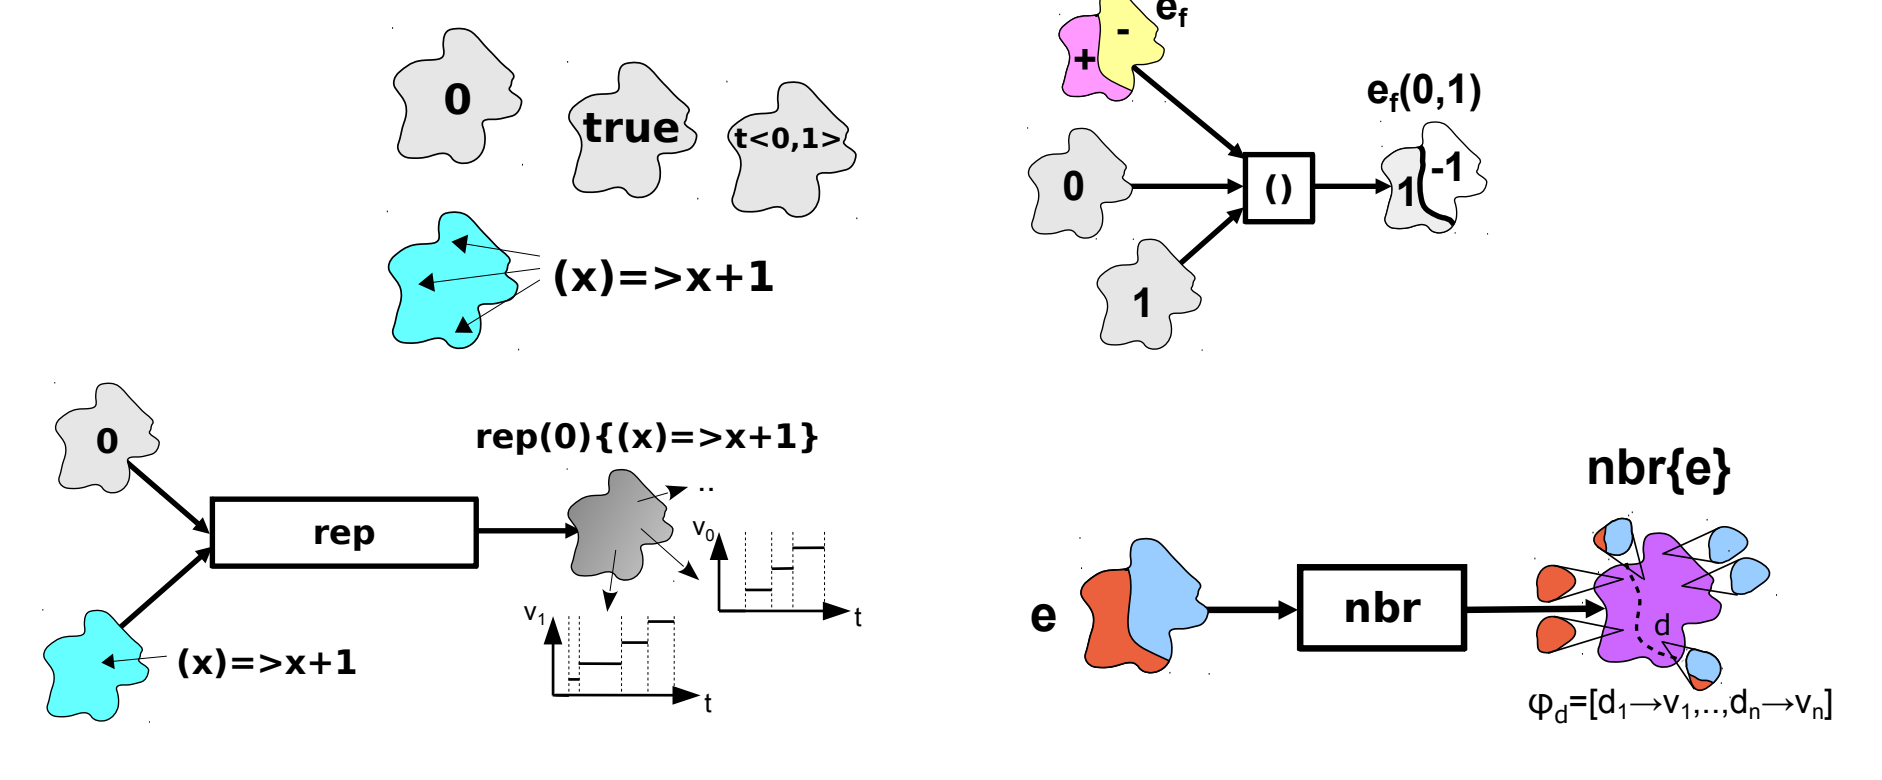
\includegraphics[width=0.8\textwidth]{img/high-level-examples.png}
\end{card}
\begin{card}[Execution Platform]
  \begin{itemize}
    \item \textbf{Requirements}:
    \begin{itemize}
      \item A notion of neighbourhood must be defined — wireless connectivity, physical proximity \dots
      \item Nodes execute in asynchronous rounds, and emit a ``round result''
      \item A node need to have recent round results of neighbours
    \end{itemize}
    \item \textbf{Execution Model}:
    \begin{enumerate}
      \item[\textbf{1}.] Retrieve context
      \item[\textbf{2}.] Aggregate program Execution
      \item[\textbf{3}.] Brodcast export to the neighbourhood
      \item[\textbf{4}.] Execute actuation (if needed)
    \end{enumerate}
    \item \textbf{NB!} the above requirements can be met by various platforms
    \begin{itemize}
      \item P2P
      \item Client-Server
      \item Edge-Cloud computing
    \end{itemize}
  \end{itemize}
\end{card}
\end{frame}
\begin{frame}{Computing with Field: mini tutorial with ScaFi}
  \begin{card}[References]
    \begin{itemize}
    \item Official Scafi on Github: \url{https://github.com/scafi/scafi}
    \item \highlight{ScafiWeb}: \url{https://scafi.github.io/web/}
    \item Official Documentation: \url{https://scafi.github.io/}
    \end{itemize}
  \end{card}
  \centering
  \cardImg{img/scafi-web.png}{0.5\textwidth}
\end{frame}
\begin{frame}{Aggregate Computing: is it expressive?}
  \begin{card}[Practically we can express]
    \begin{itemize}
      \item Complex spreading / aggregation / decay functions~\cite{beal2015aggregate-programming}
      \item Spatial leader election, partitioning, consensus~\cite{damiani2015code}
      \item Distributed spatio-temporal sensing~\cite{viroli2016execution}
      \item Splitting in parallel independent subprocesses~\cite{viroli2016execution}
      \item Dynamic deployment/spreading of code~\cite{damiani2015code}
      \item ``Collective teams'' forming based on the selected codee~\cite{viroli2015multi} \dots
      \item \dots but how to engineer complex apps out of basic constructs?
    \end{itemize}
  \end{card}
\end{frame}
\begin{frame}{GCT as a combinator set}
  \centering
  \cardImg{img/gct.png}{0.7\textwidth}
  \begin{cardTiny}
    \begin{itemize}
      \item \textbf{G}: Spreads and en-route computes information outwards a source
      \item \textbf{C}: Collects and en-route aggregates information inwards a destination
      \item \textbf{T}: Locally iterates computations (with termination)
    \end{itemize}
  \end{cardTiny}
\end{frame}
\begin{frame}{Aggregate Computing Full stack API}
  \centering
  \cardImg{img/full-stack.png}{0.5\textwidth}
\end{frame}
\begin{frame}[allowframebreaks]{Aggregate Computing current status}
  \begin{card}[Main results]
    \begin{itemize}
      \item \textbf{Formal properties}:
      \begin{itemize}
        \item self-stabilisation~\cite{viroli2018selfstab} \faArrowRight\, resilience to occasional changes
        \item eventual consistency~\cite{10.1145/3105758}
      \end{itemize}
      \item Space-Time Universality~\cite{audrito2018space}
      \item High-order Field-calculus~\cite{audrito2019tocl} \faArrowRight \, code mobility
      \item Toolchains (DSL \& Platforms)
      \item Concurrent Collective Activity \faArrowRight\, \emph{aggregate processes}~\cite{casadei2019coord-procs}
    \end{itemize}
  \end{card}
  \begin{card}[Research Directions]
    \begin{itemize}
      \item \highlight{Programmable Distributed schedulers}~\cite{zambonelli2021time}
      \item \highlight{Distributed \& spatial monitoring}~\cite{DBLP:journals/jss/AudritoCDSV21}
      \item \highlight{Pulverised architecture}~\cite{casadei2020pulverization}
      \begin{itemize}
        \item Pontetially integrated with Machine Learning~\cite{aguzzi2021research, aguzzi2022towards}
      \end{itemize}
    \end{itemize}
  \end{card}
  \begin{card}[Explored application]
    \begin{itemize}
      \item Crowd engineering~\cite{beal2015aggregate-programming,casadei2019fgcs}
      \item WSNs, Distributed sensing~\cite{casadei2018programming-actor-based-cas}
      \item Smart city (e.g., intelligent lighting)~\cite{pianini2021fgcs}
      \item Smart buildings~\cite{mariani2019fluidware}
      \item Industry 4.0~\cite{casadei2019scc}
      \item Swarm intelligence (robots, drones)~\cite{casadei2020eaai}
      \item Rescue scenarios~\cite{viroli2017aggregate-plans}
    \end{itemize}
  \end{card}
\end{frame}
\section{Aggregate Computing for Swarms: case studies}

\begin{frame}{Aggregate Computing for ``Swarms''}
  \begin{card}[Benefits]
    \begin{itemize}
      \item Fault-tolerant behaviours
      \item Network size-independent programs
      \item Potentially no need for central authority
      \item Enabling mechanisms:
        \begin{itemize}
          \item Aggregate processes \faArrowRight \, support concurrent \& collective activity
        \end{itemize}
    \end{itemize}
  \end{card}

  \begin{card}[Current status]
    \begin{itemize}
      \item Several simulations are performed with good results
      \item Lack of a API for expressing ``swarm'' like behaviours (e.g., flocks)
      \item Reality-gap \faArrowRight \, lack of test \emph{in vitro}
    \end{itemize}
  \end{card}

\end{frame}

\begin{frame}[allowframebreaks]{Aggregate Processess: Why and What}
  \begin{card}[Why?]
    \begin{itemize}
      \item FC is proven to be space-time universal
      \item \dots But is typically unfleasible to describe multiple \& dynamic computation
      \item[\faArrowRight] That are essential for ``Swarm''-like systems!! 
    \end{itemize}
  \end{card}
  \begin{card}[Aggregate process]
    \emph{A dynamic collection of computations} (a ``bubble'') \faArrowRight \, similar to OS processes but on aggregates
    \begin{itemize}
      \item \textbf{Features}:
      \begin{itemize}
        \item process lifecycle (\emph{generation}, \emph{shrinking},\emph{destruction})
        \item process logic
        \item process interaction
      \end{itemize}
    \end{itemize}
  \end{card}
  \begin{card}[What can we express with aggregate processes?]
    \begin{itemize}
      \item Move drones in flocking formation \dots \highlight{while also dynamically} \dots
      \item Detect or estimate something
      \item Elect leader
      \item Organise teams for missisions departing from the flock
    \end{itemize}
  \end{card}
  \centering
  \begin{multicols*}{3}
    \cardImg{img/drone-a}{0.3\textwidth}
    \cardImg{img/drone-b}{0.3\textwidth}
    \cardImg{img/drone-c}{0.3\textwidth}
  \end{multicols*}
\end{frame}
\begin{frame}[allowframebreaks]{Case studies}
  \begin{card}[Fire detection~\cite{casadei2020eaai}]
    \begin{multicols}{2}
      \begin{itemize}
        \item 200 UAVs
        \item start at a base station, 10 random waypoints, and back
        \item Aggregate computing used to detected emergence (not to steer the drones)
      \end{itemize}
      \centering
      \cardImg{img/fire-detection.png}{0.3\textwidth}
    \end{multicols}
    
    \end{card}
  \begin{card}[Wildlife Rescue~\cite{DBLP:journals/jsan/CasadeiAV21}]
    \begin{multicols*}{2}
      \begin{itemize}
        \item 80 mobiles UAVs, 20 stations and 100 animals
        \item the program influences the drone movements 
        \item the choice of healing an animal is made by stations (i.e., leaders).
      \end{itemize}
      \centering
      \cardImg{img/wild-rescue}{0.3\textwidth}
    \end{multicols*}
  \end{card}
  \begin{card}[Flocking API (Experimental)]
    \begin{multicols}{2}
      \begin{itemize}
        \item Express drones movement as a computational field
        \item High-Level \& Composable
        \item Extendible
        \item Allow complex movement pattern
        \begin{itemize}
          \item Anti-flocks
          \item Obstacle avoidance
          \item Team formation
          \item Goal seeking
        \end{itemize}
      \end{itemize}
      \centering
      \cardImg{img/flocks}{0.3\textwidth}
    \end{multicols}
  \end{card}
\end{frame}
\begin{frame}[allowframebreaks]
  \frametitle{References}
  \printbibliography
\end{frame}
\end{document}
